
% このファイルは自動生成されました。
% 親ファイル(tex_soturonhappyoルート)から \input して使用することを想定しています。
\begin{frame}{黄金分割法の収束プロセス}
  \begin{columns}
    \begin{column}{0.4\textwidth}
      \begin{itemize}
        \item \textbf{グレー領域}: 現在の探索区間
        \item \textcolor{red}{\textbf{赤丸}}: 今回の評価点
        \item \textcolor{blue}{\textbf{青丸}}: 既存の評価点
      \end{itemize}
      \vspace{1em}
      範囲が狭まるにつれ、範囲外の点は探索対象から除外（消去）されます。
    \end{column}
    \begin{column}{0.6\textwidth}
      \centering
      \only<1>{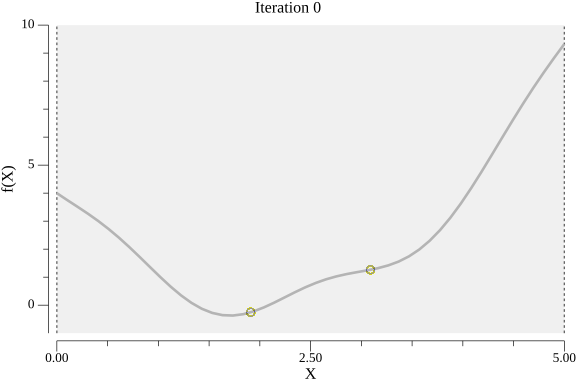
\includegraphics[width=\textwidth]{material/golden/output/golden_00.png}}
      \only<2>{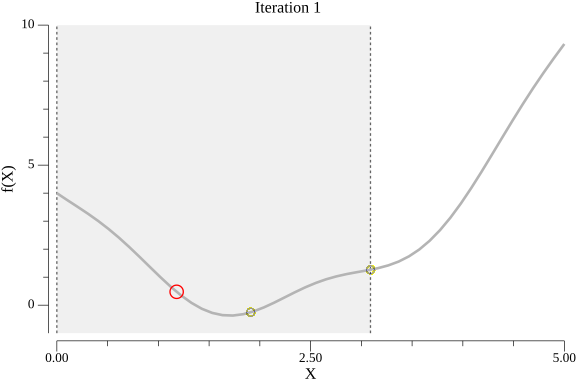
\includegraphics[width=\textwidth]{material/golden/output/golden_01.png}}
      \only<3>{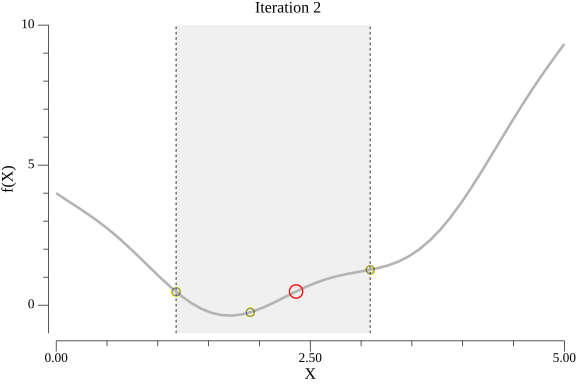
\includegraphics[width=\textwidth]{material/golden/output/golden_02.png}}
      \only<4>{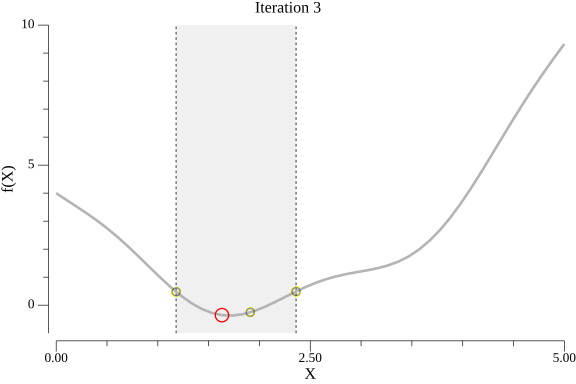
\includegraphics[width=\textwidth]{material/golden/output/golden_03.png}}
      \only<5>{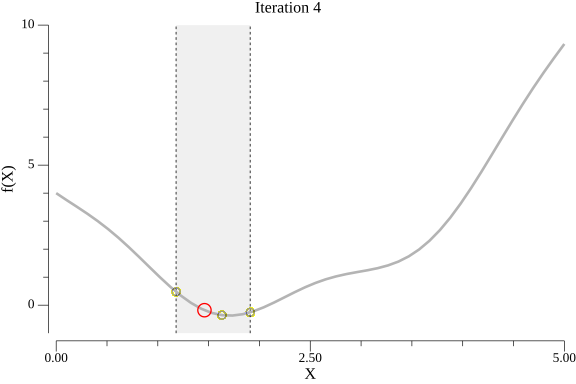
\includegraphics[width=\textwidth]{material/golden/output/golden_04.png}}
      \only<6>{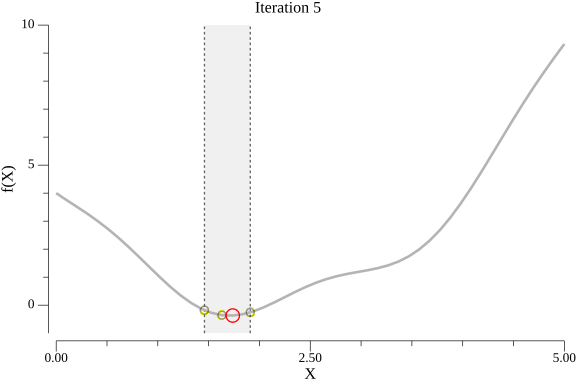
\includegraphics[width=\textwidth]{material/golden/output/golden_05.png}}
      \only<7>{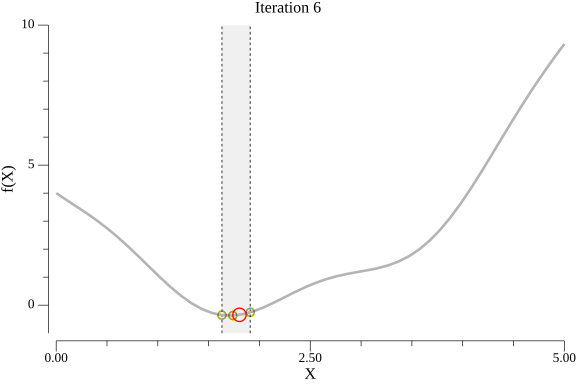
\includegraphics[width=\textwidth]{material/golden/output/golden_06.png}}
      \only<8>{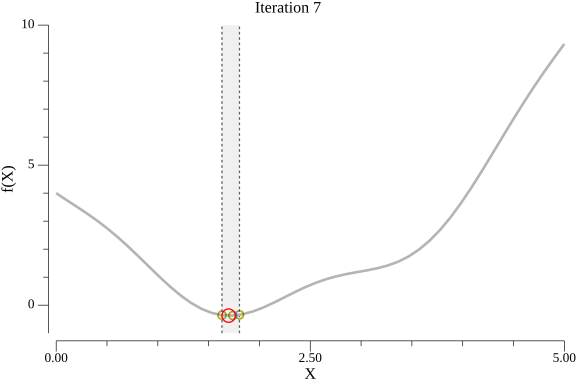
\includegraphics[width=\textwidth]{material/golden/output/golden_07.png}}
      \only<9>{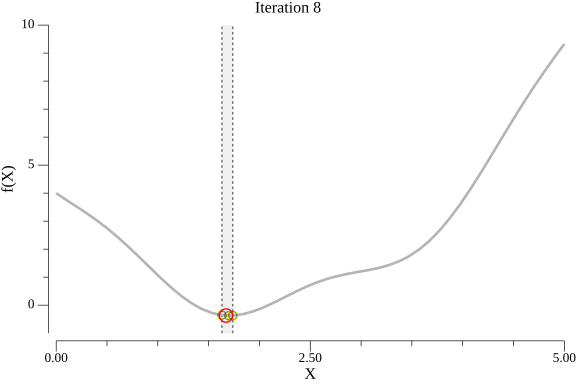
\includegraphics[width=\textwidth]{material/golden/output/golden_08.png}}
      \only<10>{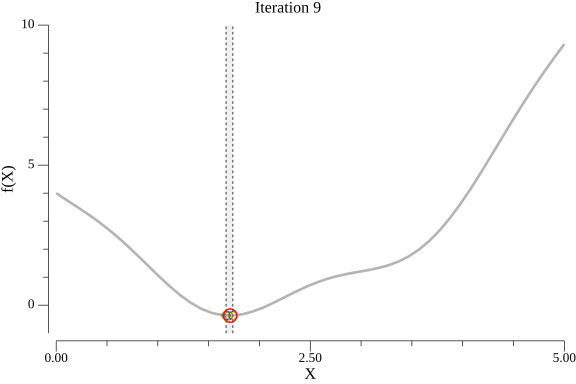
\includegraphics[width=\textwidth]{material/golden/output/golden_09.png}}
      \only<11>{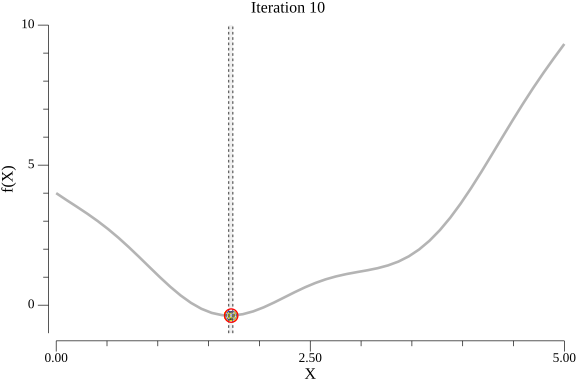
\includegraphics[width=\textwidth]{material/golden/output/golden_10.png}}
      \only<12>{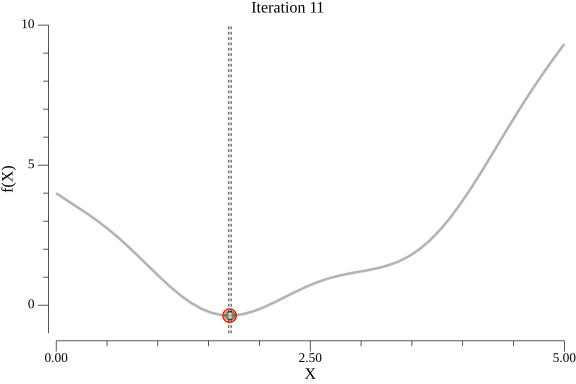
\includegraphics[width=\textwidth]{material/golden/output/golden_11.png}}
      \only<13>{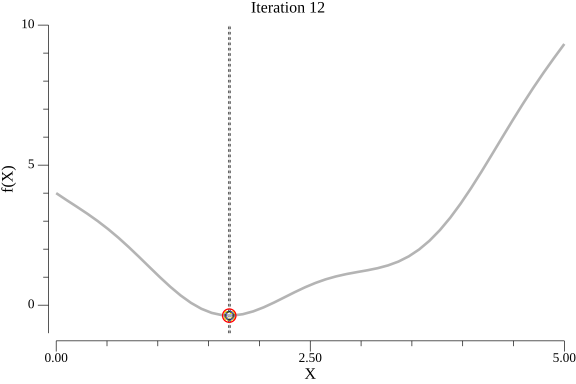
\includegraphics[width=\textwidth]{material/golden/output/golden_12.png}}
      \only<14>{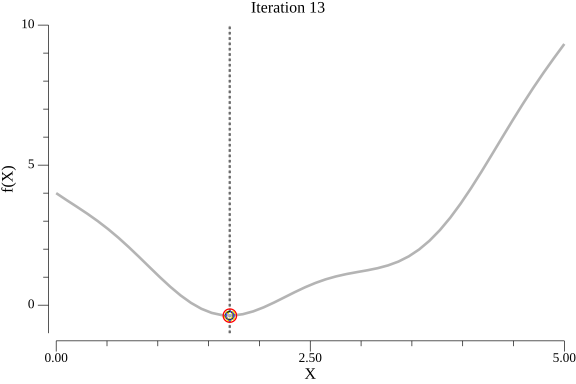
\includegraphics[width=\textwidth]{material/golden/output/golden_13.png}}
      \only<15>{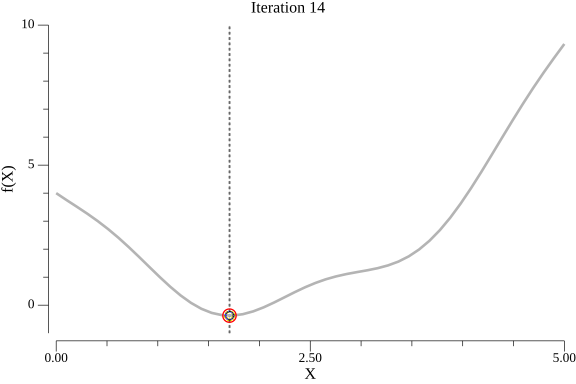
\includegraphics[width=\textwidth]{material/golden/output/golden_14.png}}
      \only<16>{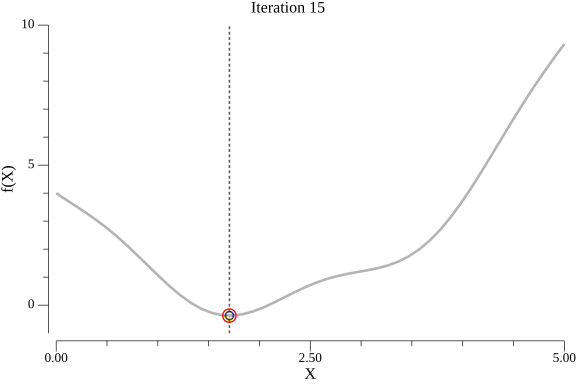
\includegraphics[width=\textwidth]{material/golden/output/golden_15.png}}
    \end{column}
  \end{columns}
\end{frame}
